\chapter{Qu'est ce que la thrombose veineuse profonde}

\section{terminologie}

On appelle thrombose le fait qu'un caillot sanguin ou thrombus se développe à l'intérieur d'un vaisseau sanguin. Il peut être soit artérielle, soit veineux. Dans les deux cas, ce caillot peut obstruer le vaisseau et donc empêcher la circulation du sang.

\begin{figure}[H]
\centering
    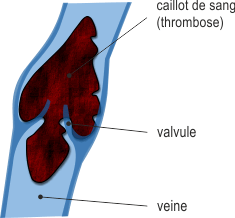
\includegraphics[scale=2,angle=0]{Images/phleb1.png}
    \caption{Exemple illustrant la thrombose.}
    \label{fig:phleb1}
\end{figure}

La phlébite correspond au cas de la thrombose veineux et plus précisément pour une veine profonde et est consécutif à l'inflammation de la veine et au risque de déplacement du caillot. D'où le terme de thrombose veineux profond DVT.

\section{Causes et conséquence}

Parmi les principales causes, nous pouvons énumérer:


\begin{itemize}
\item Une lésion dans une veine qui entraine une coagulation au niveau du tissu sanguin (blessure...).
\item Certains paramètres génétiques qui peuvent favoriser le processus de thrombose.
\item Les périodes prolongées dans une même position (alitement, accouchement, voyage long en avion...).
\item Des précédentes expériences traumatisantes pur le corps (cancer, opération...)
\item Influence de certaines substances sur la paroi des artères (tabac, médicaments...) 
\item Facteurs favorisant la formation de thrombus (obésité, diabète, hypercholestérolémie...) 
\end{itemize}

Une fois le caillot formé, il peut se produire différentes chose:

\begin{itemize}
\item Il peut de lui même se désagréger et disparaitre naturellement.
\item Il peut se calcifier ou changer de structure se qui peut amener à la formation de pelote fibreuse.
\item Il peut se détacher et atteindre un des vaisseaux pulmonaires. Ceci se traduit par une embolie pulmonaire qui s'avère très dangereuse.
\end{itemize}

Dans tous les cas, la présence de ce caillots dans le système circulatoire sanguin d'un patient peut mener à des perturbations graves du flux sanguin avec l'apparition d'oedème ou d'ulcère pour la zone inférieur du corps que nous allons étudier.


\chapter{Quels moyens de détection?}

Nous allons donner ici une liste succincte des méthodes existantes qui pourraient s'avérer utiles pour la caractérisation des caillots sanguins.

\section{Elastométrie}

L'élastométrie est une méthode d'acquisition d'image médicale non invasive très pratique car très facile à mettre en œuvre, peu couteuse en temps et en argent. Elle consiste à recréer une représentation d'une zone du corps à partir de l'élasticité du tissu biologique \cite{ophir1991elastography}.

\begin{figure}[H]
\centering
    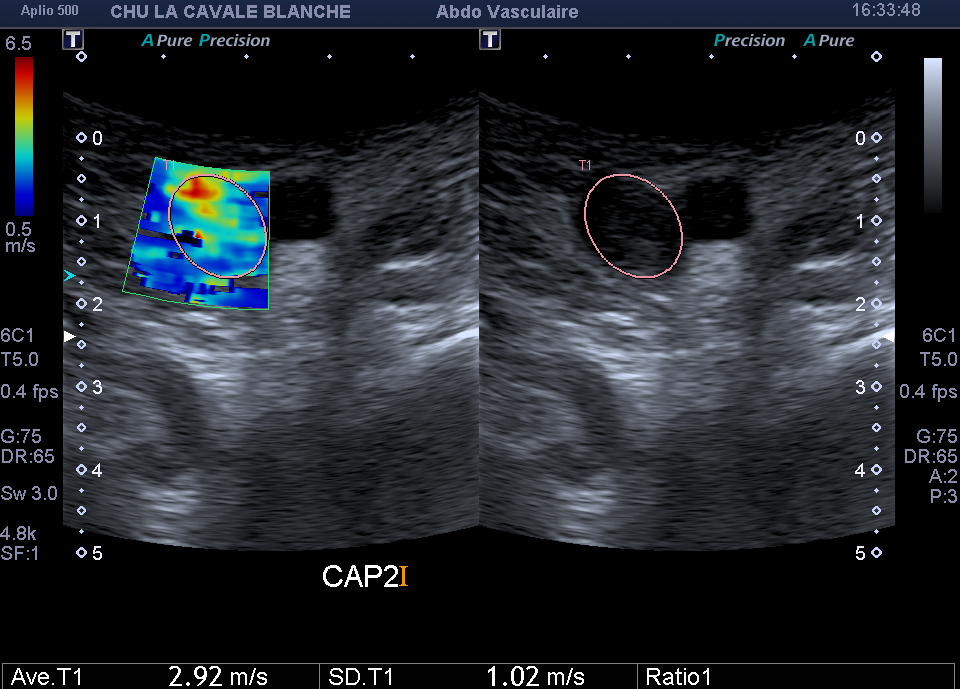
\includegraphics[scale=0.3,angle=0]{Images/ExempleElastometrie.png}
    \caption{Exemple d'image d'élastometrie.}
    \label{fig:ExempleElastometrie}
\end{figure}

En l'état, nous pouvons donner les résultats suivants:

\begin{itemize}
\item Il est toujours nécessaire de définir un protocole unique à tous les patient pour faire en sorte que les images obtenues par ce procédé soient comparables.
\item Une nouvelle sonde sera disponible dans les prochaines semaines et une partie des images vont être probablement refaites.
\item Bien que la mise en œuvre soit facile, les images obtenues sont de médiocre qualité en terme de résolution.
\end{itemize}

Pour l'instant, un doctorant cherche des pistes dans cette piste pour la détection et la caractérisation des thromboses veineuses sanguin.
 
\section{Échographie}

L'échographie est une technique d'imagerie qui consiste à utiliser des ondes ultrasons. Là encore, en fonction des propriétés du milieu, certain tissus ou partie du corps apparaitront en noir, gris ou blanc. 

\begin{figure}[H]
\centering
    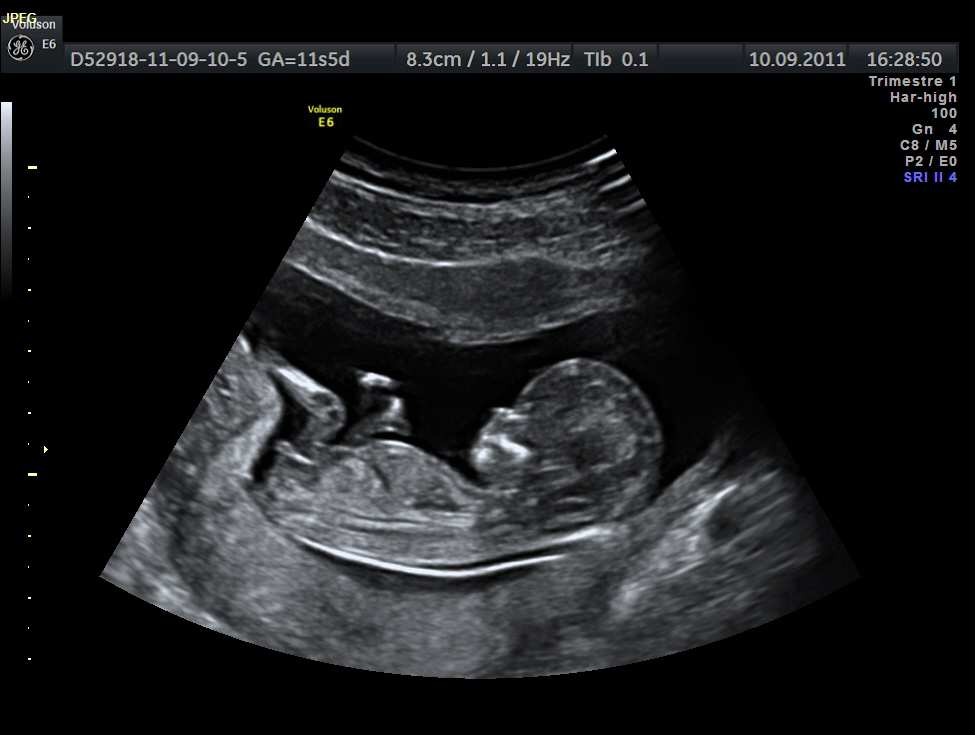
\includegraphics[scale=0.6,angle=0]{Images/Echographie-profil.jpg}
    \caption{Exemple d'image échographique pour l'obstétrie.}
    \label{fig:Echographie}
\end{figure}

Cette méthode présente les mêmes avantages. Elle est peu chère, facile à mettre en œuvre et non invasive pour le patient. Néanmoins, elle présente également des images de très faible qualité en terme de résolution.

Cette piste est également explorée pour ce projet.

\section{Computed tomography angiography / Angiographie}

L'angiographie est une technique d'imagerie qui est invasive. Bien qu'elle présente plusieurs intérêt, notamment car elle consiste à faire une imagerie des vaisseaux sanguins par rayon X (veines ou artères), il y a plusieurs effets secondaires (vomissement, vertiges, nausées, réactions allergiques, saignement important...) ou contre-indications (Grossesse, tension artérielle trop basse...). Cette piste ne sera pas étudiée ici.

\begin{figure}[H]
\centering
    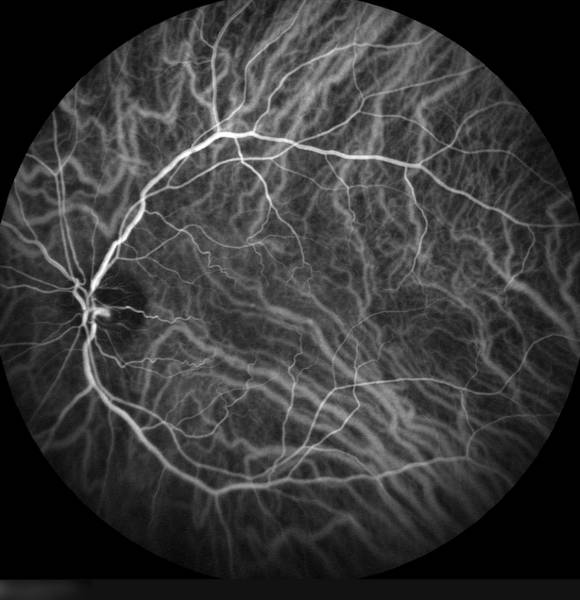
\includegraphics[scale=0.5,angle=0]{Images/m_1407858437.jpg}
    \caption{Exemple d'angiographie pour l'œil.}
    \label{fig:m_1407858437}
\end{figure}

\section{Scanner}

\textbf{Rencontre avec un médecin prévu jeudi 21 avril}

\section{IRM}

\textbf{Rencontre avec un médecin prévu jeudi 21 avril}


\chapter{Option suivie}


Dans le cadre de ce PFE, nous allons nous focaliser sur deux méthodes qui sont développées dans la thèse de M. Thatare \cite{tartare2014contribution} dans le cadre de l'aide au diagnostique du cancer de la prostate. La première va aboutir à la réalisation de carte de paramètre pharmacocinétique alors que l'autre va aboutir à faire une classification directement sur toutes les données.

\begin{figure}[H]
\centering
    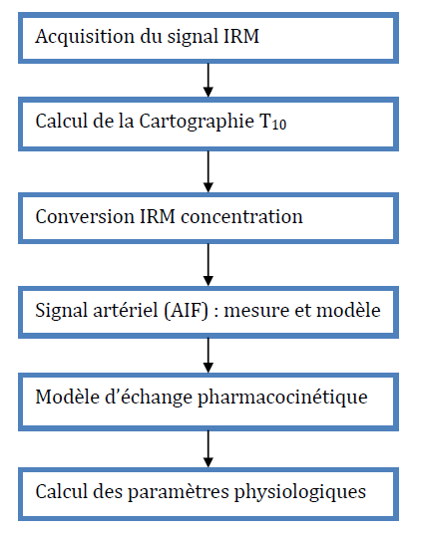
\includegraphics[scale=0.70,angle=0]{Images/MethodeTheseTartare.png}
    \caption{Méthode thèse Tartare.}
    \label{fig:MethodeTheseTartare}
\end{figure}

\pagebreak 

\section{Obtention de courbe de rehaussement à partir des IRMs de perfusion.}

La stratégie qui a été développée dans cette thèse peut être résumer en quelques lignes. Ils ont proposé d'utiliser les IRMs de perfusion, ici l'IRM T1 ou DCE-MRI, afin de décrire le fonctionnement des tissus de la zone étudiée en fonction d'une certaine caractéristique. Ici, la stratégie adoptée est de décrire la vascularisation des différents zones de la prostate car les zones tumorales ont tendance à avoir une vascularisation plus importante et donc cela va se traduire un hypo ou hyper signal sur l'IRM.

\medskip 

Le principe de l'IRM de perfusion développée ici est d'injecter un produit de contraste, ici le galonium, qui est visible par IRM et de voir comment se produit se diffuse au cours du temps dans les différentes zones du corps. A terme, nous obtenons un ensemble d'image traduisant l'évolution de la concentration du produit dans la zone étudiée au cours du temps. A partir de ceci, nous pouvons déterminer à partir de ces images la courbe d'intensité au cours du temps de chaque pixel de l'IRM. L'idée est donc de voir le comportement d'une zone du corps avant pendant et après injection de PdC.

\begin{figure}[H]
\centering
    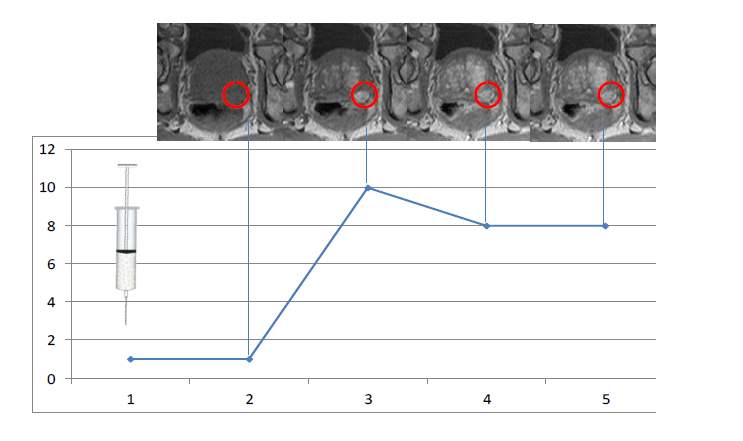
\includegraphics[scale=0.70,angle=0]{Images/ExempleCourbeDeRehaussement.png}
    \caption{Exemple courbe de rehaussement.}
    \label{fig:ExempleCourbeDeRehaussement}
\end{figure}

Plusieurs methodes d'analyse s'offre à nous à partir d'ici:

\begin{itemize}
\item Analyse qualitative: Méthode d'analyse qui consiste à regarder la forme de la courbe et en déduire "à l'œil" l'état du tissu.
\item Analyse semi-quantitative: Méthode plus rigoureuse que la précédente qui consiste à calculer le temps de pic de la courbe, le temps d'absorption et de dilution (wash-in et wash-out)... afin d'en déduire des caractéristiques sur le tissu.
\item Analyse quantitative: Méthode d'analyse beaucoup plus contraignante car elle impose de proposer un modèle qui peut caractériser les échanges entre cellules afin de traduire l'évolution de la concentration de PdC dans le tissu. Néanmoins, avec une telle méthode, nous pouvons obtenir des cartes de paramètres pharmacocinétiques qui traduisent les zones homogène dans la zone étudiée.
\end{itemize}

La méthode qui a été choisie est la méthode quantitative car elle permet d'obtenir des résultats particulièrement pertinents pour réaliser de l'aide au diagnostique.

\medskip 

Néanmoins, un gros problème reste encore à résoudre. Nous avons ici que des courbes d'intensité en fonction du temps et non pas de concentration en fonction du temps. Il faut donc encore trouver un moyen de trouver une transformation entre ces deux courbes.

Pour ce faire, il faut déterminer deux paramètres:

\begin{itemize}
\item L'AIF: Fonction d'entré artérielle. Cette fonction fait référence à la concentration de PdC dans le vaisseau alimentant le tissu étudié. Il faut donc détecter quelle est l'artère alimentant le tissu, l'isoler estimer cette fonction à partir de la courbe de rehaussement de tous les points appartenant à la veine.
\item T10: Temps de relaxation longitudinal au temps zéro. Cette constante de temps est fortement liée au temps de réponse du tissu à la perturbation engendrée par l'injection de produit de contraste.
\end{itemize}

Avec ces deux paramètres, il est possible de passer de la courbe de intensité au cours du temps à la courbe concentration au cours du temps. Ces courbes sont ensuite approximées par des expressions théoriques qui correspondent à des modèles. On peut donc en déduire quels sont les valeurs des différents paramètres qui permettent d'interpoler ces courbes et ainsi réaliser des cartes de paramètre pharmacocinétique. L'autre possibilité est de faire une classification sur les différentes courbes de concentration directement.


\section{Carte de paramètre pharmacocinétique.}

A partir du travail qui a été réalisé au-dessus, il nous est possible de faire des cartes montrant les variations des valeurs des paramètres pharmacocinétiques. L'idée est de récupérer les valeurs des paramètres qui permettent d'interpoler les courbes de concentration en fonctions du temps et de voir quelles sont les zones de la prostate qui présentent les même propriété.

\medskip 

Le modèle utilisé dans cette thèse est appelé modèle de Toft et on parvient au final à des cartes comme ci-dessous \ref{fig:CarteDeParametresPharmacocinetique}.

\begin{figure}[H]
\centering
    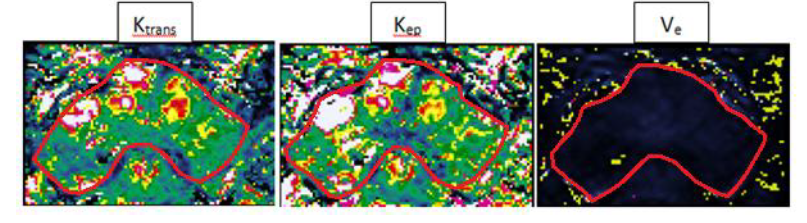
\includegraphics[scale=0.7,angle=0]{Images/CatreDeParametresPharmacocinetique.png}
    \caption{Carte de parametres pharmacocinetiques.}
    \label{fig:CarteDeParametresPharmacocinetique}
\end{figure}

La figure qui suit \ref{fig:ExempleApplication} montre un exemple d'application particulièrement parlant. L'IRM de gauche représente l'IRM de perfusion sous angle T1, l'IRM de droite représente l'IRM de perfusion sous angle T2 et la carte à droite représente les différentes lésions de la prostate après analyse par un médecin. Au final, La carte obtenue par le paramètre $K_{trans}$ permet d'identifier de façon très claire une des lésions de la prostate du patient.

\begin{figure}[H]
\centering
    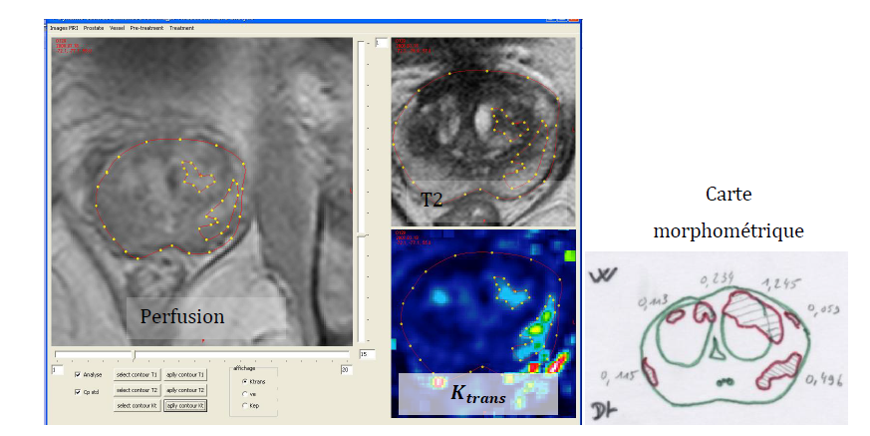
\includegraphics[scale=0.6,angle=0]{Images/ExempleApplication.png}
    \caption{Exemple de carte de parametres pharmacocinetiques.}
    \label{fig:ExempleApplication}
\end{figure}

\section{Classification des courbes de rehaussement à partir de la classification spectrale.}

Autre méthodologie développée pour réaliser des programmes d'aide au diagnostique consiste à réaliser une classification ou des clusters des différentes courbes d'intensité obtenues afin d'isoler les courbes présentant le même comportement entre elles. Ainsi, on obtient une nouvelle carte segmentée qui indique les régions qui présentent les même caractéristiques, ici la vascularisation.

\medskip

La figure qui suit montre la méthodologie appliqué ici \ref{fig:Classif}.
 
\begin{figure}[H]
\centering
    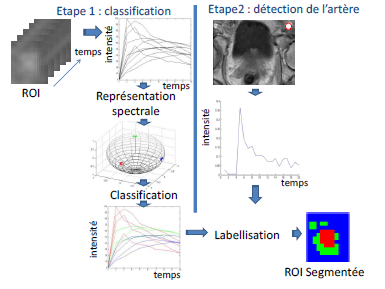
\includegraphics[scale=1,angle=0]{Images/Classif.png}
    \caption{Méthodologie suivie pour la classification.}
    \label{fig:Classif}
\end{figure}

La présente thèse utilise la classification spectrale car elle est particulièrement adaptée aux types d'entrées (signaux temporels) que nous avons ici. La partie suivante va détailler en profondeur cette théorie. Dans le cadre de cette thèse, il réalise une classification des différents signaux en trois classes et il parvienne à obtenir une image segmentée où les zones tumorales sont clairement identifiables.

\medskip

La figure qui suit \ref{fig:ResultatAlgo} montre le résultats de la classification sur des données simulées. Comme on peut le voir, le programme est très performant.

\begin{figure}[H]
\centering
    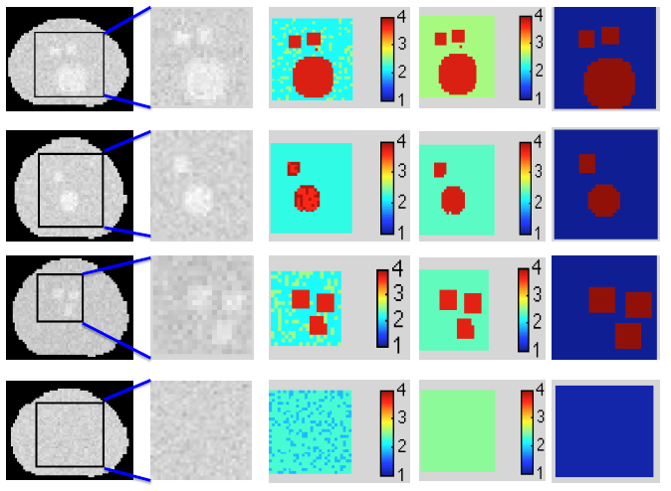
\includegraphics[scale=0.5,angle=0]{Images/ResultatAlgo.png}
    \caption{Dans l'ordre, - prostate avec présence ou non de tumeur - zoom sur la région d'intérêt - résultat de l'algorithme de classification - fusion de l'information en un résultat zone saine / zone tumorale - table de vérité.}
    \label{fig:ResultatAlgo}
\end{figure}

Dans le cadre de la lutte contre le cancer prostatique, le précédent programme permettait d'avoir une segmentation d'image automatique assez performant mais qui montrait des très bons résultats lorsqu'il était couplé à d'autres méthodes  d'aide au diagnostique.

\chapter*{Conclusion}

La partie que nous venons de voir présente beaucoup de piste intéressante pour les objectif que nous poursuivons. Néanmoins, cette méthodologie ne pourra pas être réutilisé tel quel pour le thrombose veineuse profonde. Néanmoins, plusieurs étapes comme l'extraction de signaux temporelle à partir d'IRMs de perfusion, la classification spectrale ou l'extraction de paramètres physiologiques peuvent s'avérer particulièrement pertinent tant pour ce projet que pour d'autre enjeux médicaux (cancer du sein...).



